%%%%%%%%%%%%%%%%%%%%%%%%%%%%%%%%%%%%%%%%%%%%%%%%%%%%%%%
%%% LATEX FORMATTING - LEAVE AS IS %%%%%%%%%%%%%%%%%%%%
\documentclass[11pt]{article} % documenttype: article
\usepackage[top=20mm,left=20mm,right=20mm,bottom=15mm,headsep=15pt,footskip=15pt,a4paper]{geometry} % customize margins
\usepackage{times} % fonttype
\usepackage{url}
\usepackage{graphicx}
\usepackage{subcaption}
\usepackage{amsmath}
\usepackage{listings}
\makeatletter         
\def\@maketitle{   % custom maketitle 
\begin{center}
{\bfseries \@title}
{\bfseries \@author}
\end{center}
\smallskip \hrule \bigskip }
\graphicspath{ {../results} }

%%%%%%%%%%%%%%%%%%%%%%%%%%%%%%%%%%%%%%%%%%%%%%%%%%%%%%%%%%%%%%%%%%%%
%%% MAKE CHANGES HERE %%%%%%%%%%%%%%%%%%%%%%%%%%%%%%%%%%%%%%%%%%%%%%
\title{{\LARGE Machine Learning in Natural Language Processing: \newline Assignment 2}\\[1.5mm]} % Replace 'X' by number of Assignment
\author{Shifei Chen} % Replace 'Firstname Lastname' by your name.

%%%%%%%%%%%%%%%%%%%%%%%%%%%%%%%%%%%%%%%%%%%%%%%%%%%%%%%%%%%%%%%%%%%%
%%% BEGIN DOCUMENT %%%%%%%%%%%%%%%%%%%%%%%%%%%%%%%%%%%%%%%%%%%%%%%%%
%%% From here on, edit document. Use sections, subsections, etc.
%%% to structure your answers.
\begin{document}
\maketitle

\section{Implementing Missing Bits}

\subsection{Gradient Decent Calculation}
The frist part we were going to do is to implement the gradient decent calculation. Based on the formula $w \leftarrow w - \eta\nabla f(w,b;\tau)$ and $b \leftarrow b - \eta\nabla b$ where $\eta$ means the learning rate and $\nabla f(w,b;\tau)$ and $\nabla b$ means the gradient of the weight and the bias. Luckily the function \verb|gradient_descent_step()| already provided us all of the ingredients in its parameter list. One thing to notice is that since the \verb|old_weights| and \verb|weight_grads| are both vectors (or \verb|list|s in Python) we can't multiply them directly to the learning rate. The lab instruction mentioned to use \verb|zip()| as a simple solution to vector calculation and I found it to be useful here indeed.

\subsection{Hinge Loss Calculation}

The next missing block is the Hinge Loss funciton. For the actual loss calculation it took me a while to fully understand the formula whose $y^{(i)}$ and $x^{(i)}$ mean the $i$th dimension of the label and the data. Then calculating  $y^{(i)}(w\cdot x^{(i)} + b)$ is also not as intuitive as it looks because of the way the data was stored. Recall how the dot product of two vectors works, e.g. $\left(\begin{smallmatrix}a\\b\end{smallmatrix}\right) \cdot \left(\begin{smallmatrix}c\\d\end{smallmatrix}\right) = a\times c + b\times d$, we need to find out the sum of the product of all $i$ dimensions, $\sum_{i=1}^{|\tau|}{w^{(i)}\times x^{(i)}}$, so if either $w^{(i)}$ or $x^{(i)}$ is $0$ the whole term can be ignored. In our case the features were stored in a sparse representation and its corresponding label is always $1$ or $-1$, we just need to find out whether the features are positive or negative and sum up all of them to calculate $y^{(i)}(w\cdot x^{(i)} + b)$. After that check if the result is smaller than $1$ and put it inside a loop we will get the final loss. 

The gradient of the loss function was also very similar once I have figured out how to calculate with a sparsely representated data.

\subsection{L2 Regulariser Calculation}

The definition is ``The 2-norm is equal to the square root of the sum of the squared vector components'' so it was straightforward, though we usually drop the square root in practice.

\section{Exploring hyperparameters}

\subsection{Learning Rate \& Number of Iterations}

The default number of iterations 5 is way too small to do any meaningful observations. My initial trial increased it to 50 and I found the learning curve was still a straight line, like the left one in Figure 1. Also the accuracy on both the training set and the validation set were low, only at around 70\% so I decided to increase the learning rate to 0.08 and make the program to learn deeper (200 iterations) in the next trial.

The result was better for certain as shown on the right picture in Figure \ref{fig:learning_rate}, but interestingly during the first 20 iterations the accuracy on the validation set was jumping between 0.48 and 0.515, as the zigzags in the begining of the learning curve. i realized this is the case where my learning rate was set too high. Also after around 100 iterations the accuracy on the validation set stucked at 0.875 so half the number of itertaions to 100 seemed to be a good idea as it wouldn't benefit a lot after 100 iterations. Then after some tweaking and tuning I found 0.07 was the largest learning rate to get a smooth learning curve.

\begin{figure}[p]
    \centering
    \begin{subfigure}{0.4\textwidth}
        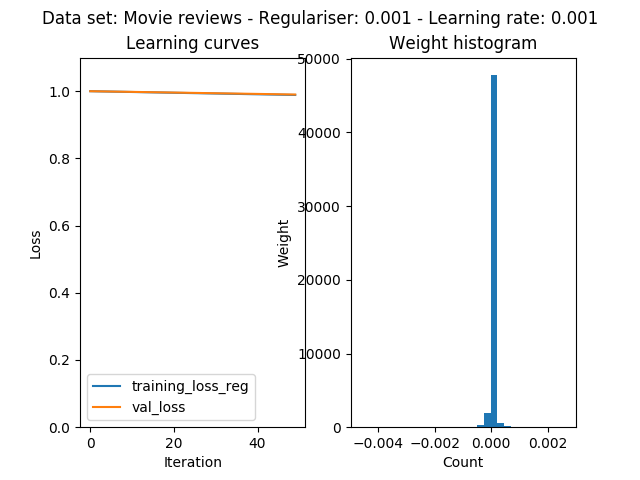
\includegraphics[width=\columnwidth, keepaspectratio]{{../results/0.001_50_l1_0.001_log}.png}
    \end{subfigure}
    \begin{subfigure}{0.4\textwidth}
        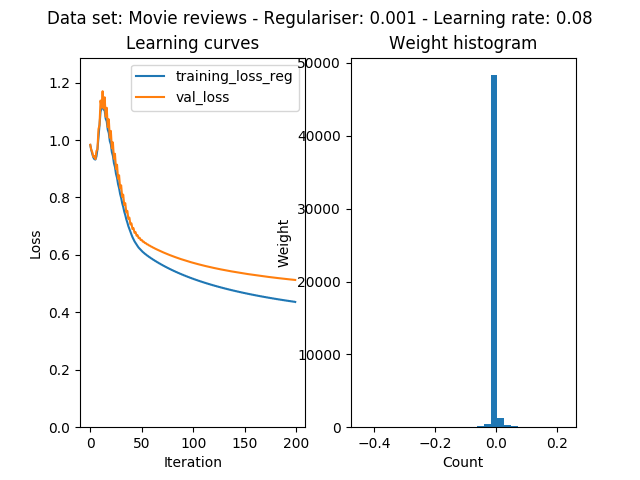
\includegraphics[width=\columnwidth, keepaspectratio]{{../results/0.08_200_l1_0.001_log}.png}
    \end{subfigure}
    \caption{Learning Curves Showing Different Learning Rates and Number of Iterations}
    \label{fig:learning_rate}
\end{figure}

\subsection{Regularization}

L2 regularization performed better than L1. In Figure \ref{fig:l1} and \ref{fig:l2} we can see that L1 regulariser has higher loss than L2 regardless of the $\lambda$ value. Also L1 was more sensitive to high regularization strength. When $\lambda$ was set to 0.003 the learning curve in L1 shows unsmoothness and it becomes significnt when $\lambda=0.01$.

Within the L2 regulariser, different regularization strength has a minor effect on the loss and the accuracy. I can only see the difference between $\lambda=0.001$, $0.002$ and $0.003$ by overlaying the learning curves together and it shows when $\lambda=0.001$ the classifier has the lowerest loss.

Therefore based on the fact that L2 regulariser performed better than L1 and the $\lambda$ value doesn't change the learning curve a lot, I decided to stop exploring other weaker regularization strengths and stick with L2 when $\lambda=0.001$ for future experienments.

\begin{figure}[p]
    \centering
    \begin{subfigure}{0.4\textwidth}
        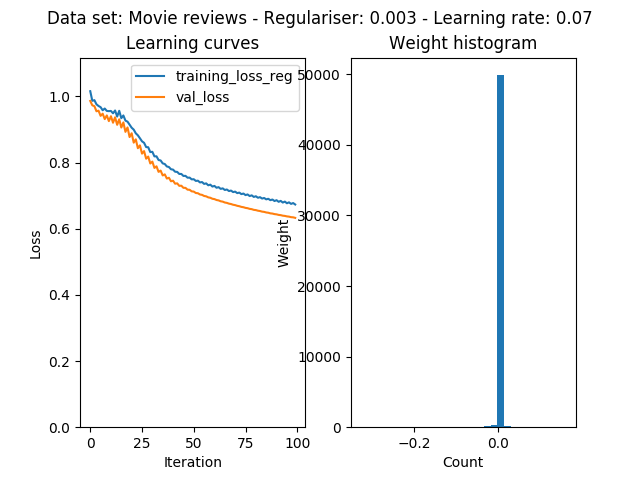
\includegraphics[width=\columnwidth, keepaspectratio]{{../results/0.07_100_l1_0.003_log}.png}
    \end{subfigure}
    \begin{subfigure}{0.4\textwidth}
        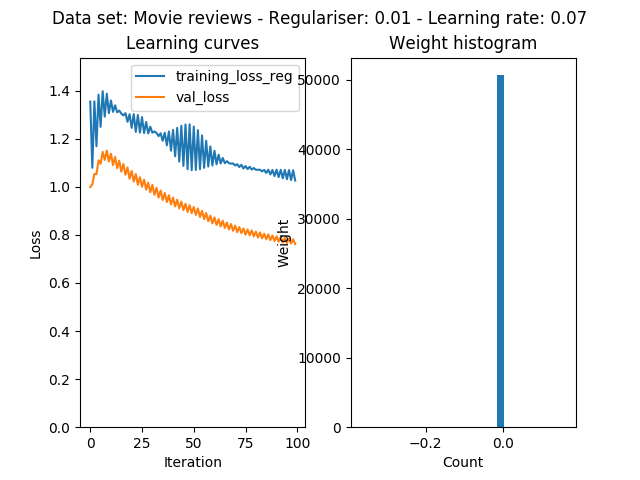
\includegraphics[width=\columnwidth, keepaspectratio]{{../results/0.07_100_l1_0.01_log}.png}
    \end{subfigure}
    \caption{Learning Curves Showing Different Regularization Strength in L1}
    \label{fig:l1}
\end{figure}
\begin{figure}[p]
    \centering
    \begin{subfigure}{0.4\textwidth}
        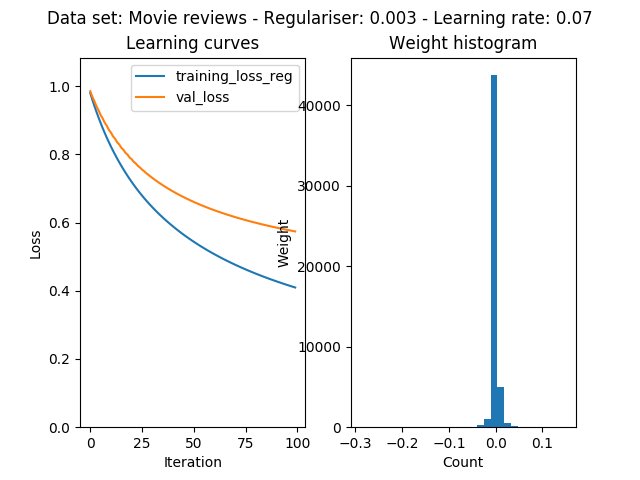
\includegraphics[width=\columnwidth, keepaspectratio]{{../results/0.07_100_l2_0.003_log}.png}
    \end{subfigure}
    \begin{subfigure}{0.4\textwidth}
        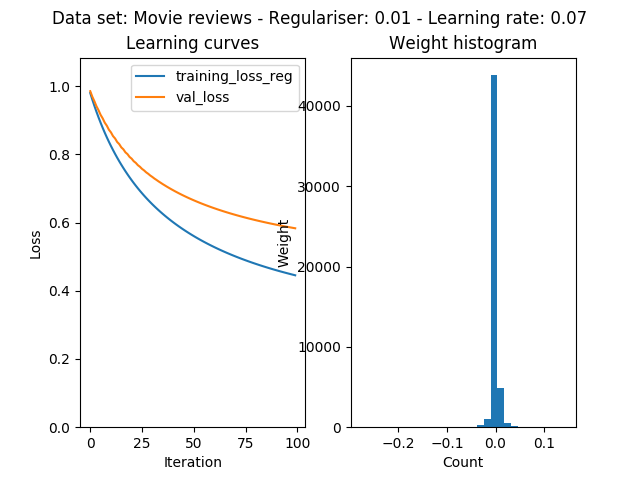
\includegraphics[width=\columnwidth, keepaspectratio]{{../results/0.07_100_l2_0.01_log}.png}
    \end{subfigure}
    \begin{subfigure}{0.4\textwidth}
        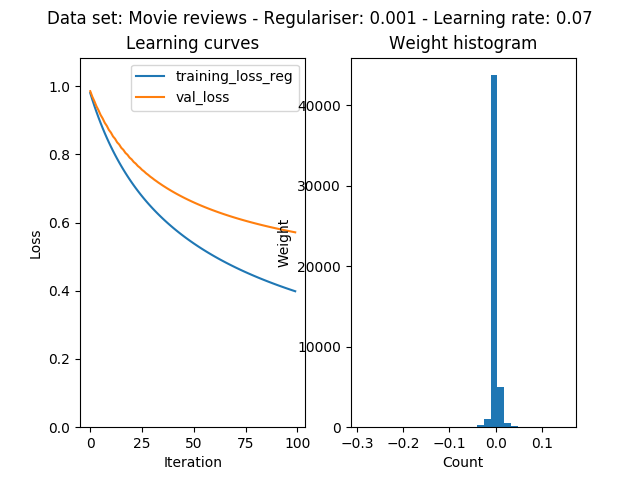
\includegraphics[width=\columnwidth, keepaspectratio]{{../results/0.07_100_l2_0.001_log}.png}
    \end{subfigure}
    \begin{subfigure}{0.4\textwidth}
        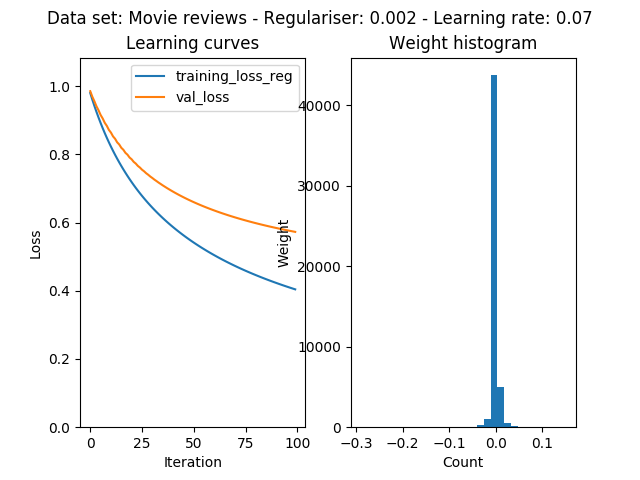
\includegraphics[width=\columnwidth, keepaspectratio]{{../results/0.07_100_l2_0.002_log}.png}
    \end{subfigure}
    \caption{Learning Curves Showing Different Regularization Strength in L2}
    \label{fig:l2}
\end{figure}

\subsection{Loss Function}

Change the loss function from logistic loss to hinge loss does change the learning rate quite a lot. In figure \ref{fig:log_and_hinge} if we carry the same learning rate from logistic loss to hinge loss the learning curve will become rough and not convex everywhere any more. Eventually I lowered the learning rate to 0.02 to make it smooth and convex again. 

To see the possible higher accuracy after longer iterations, I increased the number of iterations to 500 and it dropped slightly to 0.87 but surprisingly the curve became rough again. I also re-ran the classifier using the logistic loss function and its best learning rate for 500 iterations, which achieved an accuracy of 0.88 on validation data and stays smooth.

\begin{figure}[p]
    \centering
    \begin{subfigure}{0.4\textwidth}
        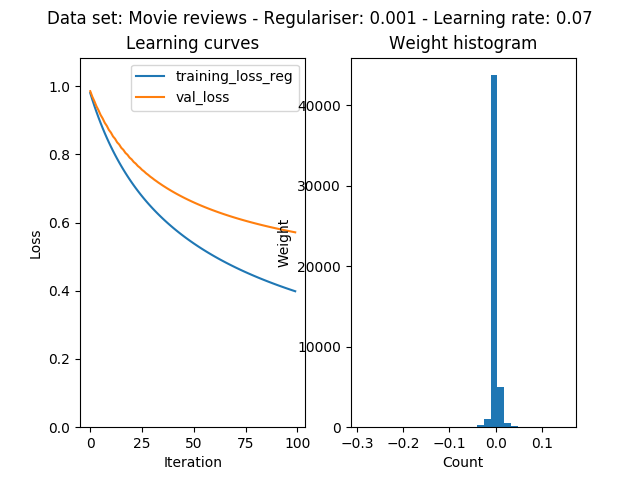
\includegraphics[width=\columnwidth, keepaspectratio]{{../results/0.07_100_l2_0.001_log}.png}
        \caption{Logistic Loss}
    \end{subfigure}
    \begin{subfigure}{0.4\textwidth}
        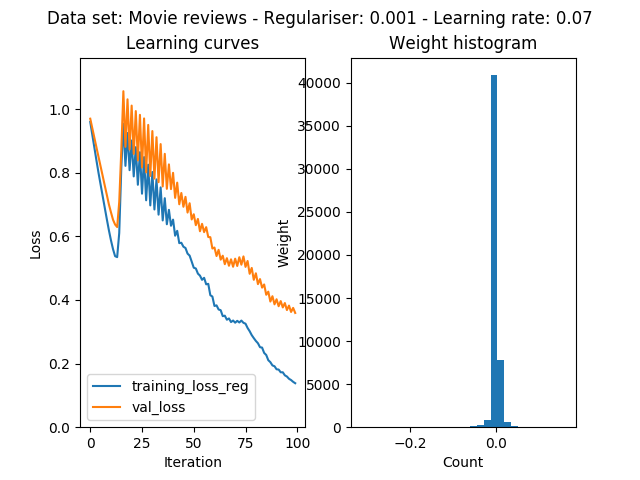
\includegraphics[width=\columnwidth, keepaspectratio]{{../results/0.07_100_l2_0.001_hinge}.png}
        \caption{Hinge Loss}
    \end{subfigure}
    \caption{Learning Curves Showing Different Loss Functions}
    \label{fig:log_and_hinge}
\end{figure}

\begin{figure}[p]
    \centering
    \begin{subfigure}{0.4\textwidth}
        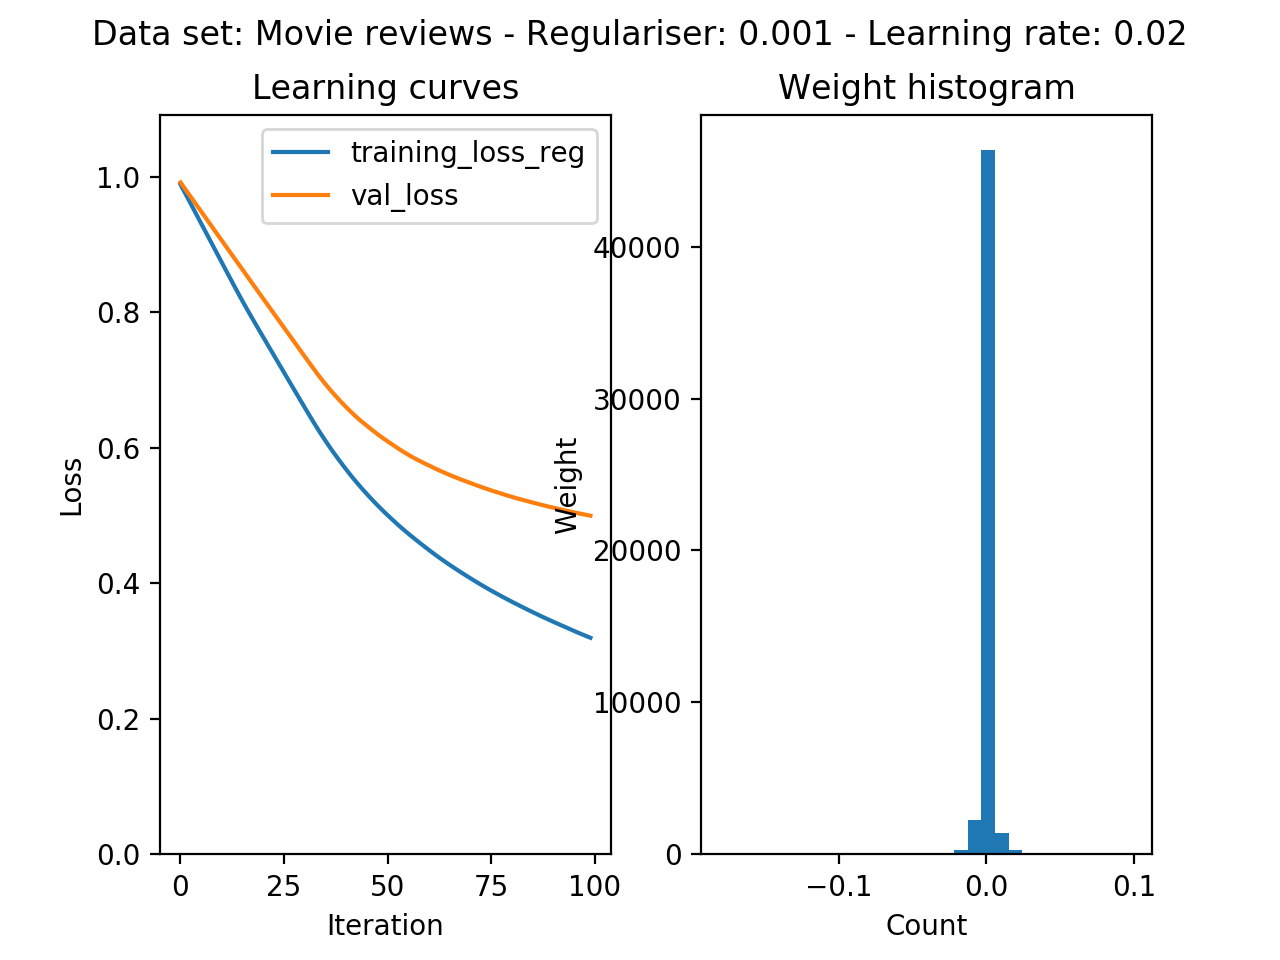
\includegraphics[width=\columnwidth, keepaspectratio]{{../results/0.02_100_l2_0.001_hinge_0.87}.png}
    \end{subfigure}
    \begin{subfigure}{0.4\textwidth}
        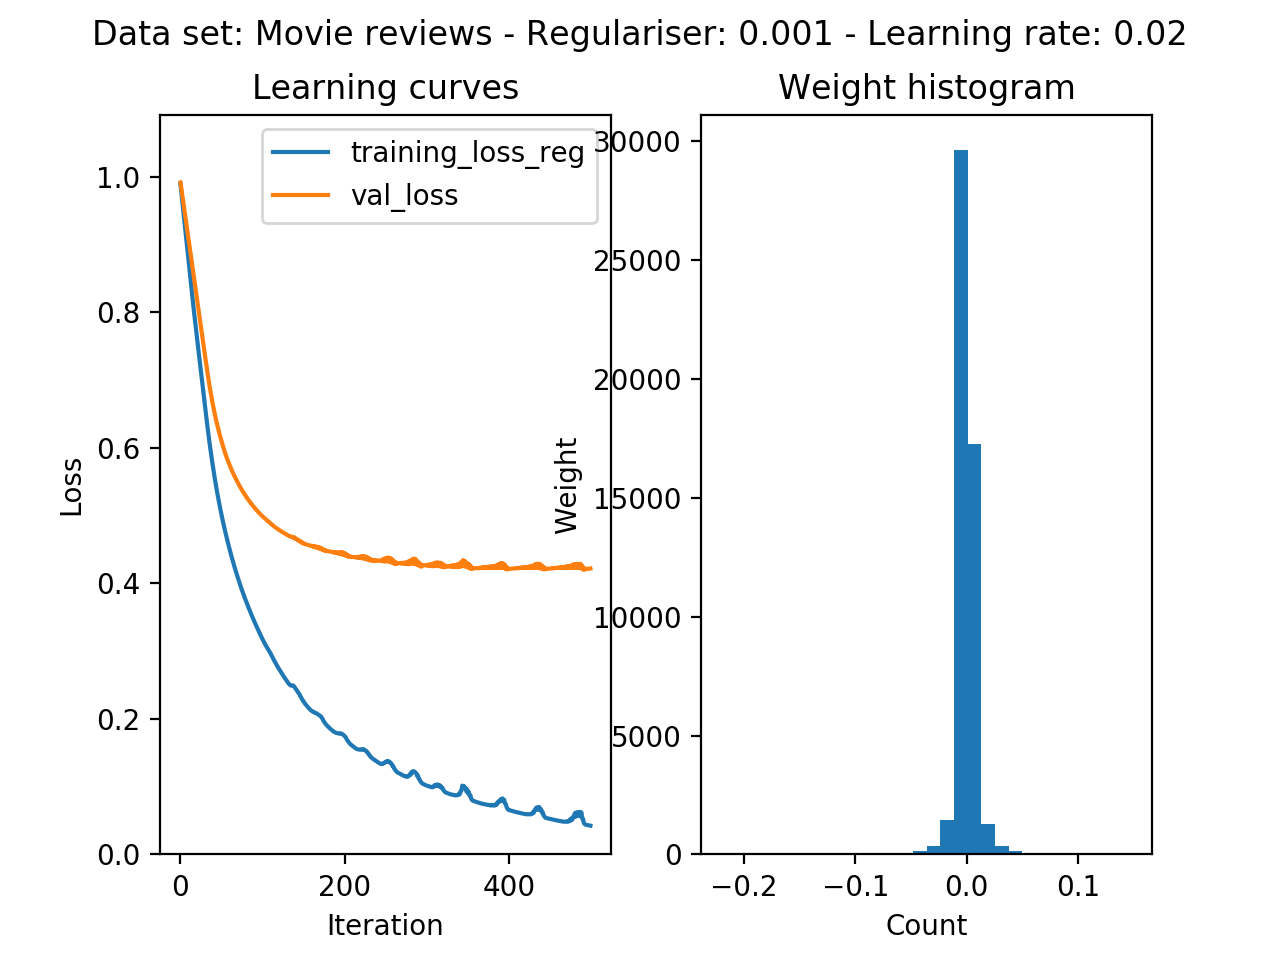
\includegraphics[width=\columnwidth, keepaspectratio]{{../results/0.02_500_l2_0.001_hinge_0.855}.png}
    \end{subfigure}
    \caption{Learning Curves Showing Results of Hinge Loss after Longer Iterations}
    \label{fig:hinge_convex}
\end{figure}

\subsection{Conclusion}

We can choose most of the hyperparameters by looking at the learning curve. Within the same number of iterations, a high learning rate would result in a rough curve with lots of zigzags while a very low learning rate will draw a straight line instead a curve. Also the number of iterations initially shouldn't be a tiny number at first otherwise you will always get a straight line, after that you can decrease it by observing from which iteration the accuracy stays.

L2 Regularization performed better than L1. Changing the regularization strength shortens the distance between training loss and validation loss, though on L2 it didn't differ much. 

Different loss functions have different best learning rates. Hinge loss are more likely to introduce rough and concave learning curves. I think it corresponds to the feature of its formula as it never punishes positive predictions whose margin is larger than 1. There for it's very like that in our binary scenario the objective function will not learn if it meets several correct sample in serial and suddenly changed a lot if it meets a incorrect one.
For this reason, logistic loss is more perferable on this data set.

The complete result between different combinations of hyperparameters is shown in the table below. My final set of hyperparameters are
\begin{lstlisting}[language=Python]
    reg_lambda = 0.001
    learning_rate = 0.03
    niterations = 100
    loss_function = LogisticLoss()
    regulariser = L2Regulariser()
\end{lstlisting}
which achieved 0.89 in accuracy and 0.570501 in loss on the test data set.

\begin{table}[h]
    \begin{center}
        \label{tab:table1}
        \begin{tabular}{c|c|c|c|c|c|c}
            \textbf{Learning Rate} & \textbf{Iterations} & \textbf{Regulariser} & \textbf{Strength} & \textbf{Loss Function} & \textbf{Loss} & \textbf{Accuracy}\\
            \hline
            0.001 & 50 & L1 & 0.001 & Logistic & 0.989857 & 0.715\\
            0.08 & 200 & L1 & 0.001 & Logistic & 0.51278 & 0.875\\
            0.07 & 100 & L1 & 0.001 & Logistic & 0.592087 & 0.87\\
            0.06 & 100 & L1 & 0.001 & Logistic & 0.610456 & 0.87\\
            0.07 & 100 & L1 & 0.003 & Logistic & 0.633021 & 0.84\\
            0.07 & 100 & L2 & 0.001 & Logistic & 0.571249 & 0.885\\
            0.07 & 100 & L2 & 0.01 & Logistic & 0.583123 & 0.885\\
            0.07 & 100 & L2 & 0.006 & Logistic & 0.577885 & 0.885\\
            0.07 & 100 & L2 & 0.003 & Logistic & 0.573915 & 0.885\\
            0.07 & 100 & L2 & 0.001 & Hinge & 0.359204 & 0.875\\
            0.04 & 100 & L2 & 0.001 & Hinge & 0.45165 & 0.815\\
            0.03 & 100 & L2 & 0.001 & Hinge & 0.457777 & 0.86\\
            0.02 & 100 & L2 & 0.001 & Hinge & 0.49974 & 0.87\\
            0.02 & 100 & L2 & 0.01 & Hinge & 0.503129 & 0.87\\
            0.03 & 100 & L2 & 0.01 & Hinge & 0.46325 & 0.845\\
            0.02 & 100 & L2 & 0.003 & Hinge & 0.500433 & 0.87\\
            0.02 & 500 & L2 & 0.001 & Hinge & 0.49974 & 0.87\\
            0.07 & 500 & L2 & 0.001 & Logistic & 0.447934 & 0.88\\
        \end{tabular}
        \caption{Classifiers' Performance with Different Sizes of Data}
    \end{center}
\end{table}

\section{Perceptron Learning Algorithm}

Implementing the algorithm is very similar to the implementation of the missing bits before. Be aware that $w\cdot x$ means two vectors doing the dot product and the sparse representation in the training data. I have spent more time on integrating the algorithm into the \verb|main()| function instead. The Perceptron Algorithm doesn't require any gradient, regularization or loss calculation so I have removed all these unnecessary parameters, setting unused log records to 0 (removing them will cause an exception in the \verb|util.py|).

When I ran the Perceptron Algorithm I found it can get an accuracy of 0.83 on the validation set, but a higher 0.87 on the test set. Also I have noticed that it took much less steps to converge--in 13 steps the accuracy on the training will converge to 1 and all the rest steps will not improve that any more. In this situation the classifier will not get updated since the algorithm is designed to update the weights and the bias only when it made wrong predictions. Therefore I have also put a line of code to tell the classifier to stop when it reaches 100\% accuracy on the training set.

Perceptron Algorithm is a very simple yet efficient algorithm to solve binary classification. The calculation is not complicated and saves lots of time compared to the gradient decent algorithm if the data set has a linear border between positive and negative.

\end{document}